\documentclass{article}
\usepackage[utf8]{inputenc}

\title{Laboratorio01U2_INTELIGENCIA_NEGOCIOS}
\author{edwartbalcon}
\date{Septiembre 2021}

\usepackage[utf8]{inputenc}
\usepackage[spanish]{babel}
\usepackage{natbib}
\usepackage{graphicx}

\begin{document}

\title{Caratula}

\begin{titlepage}
\begin{center}
\begin{Large}
\textbf{UNIVERSIDAD PRIVADA DE TACNA} \\
\end{Large}
\vspace*{-0.025in}
\begin{figure}[htb]
\begin{center}

\includegraphics[width=6cm]{./images/logo_UPT}
\end{center}
\end{figure}
\vspace*{-0.025in}
\begin{Large}
\textbf{FACULTAD DE INGENIERIA} \\
\end{Large}
\vspace*{0.05in}
\begin{Large}
\textbf{Escuela Profesional de Ingeniería de Sistema} \\
\end{Large}


\vspace*{0.4in}

\vspace*{0.1in}
\begin{Large}
\textbf{Informe de laboratorio 01: Modelamiento Dimensional} \\
\end{Large}

\vspace*{0.3in}
\begin{Large}
\textbf{Curso: Inteligencia de negocios} \\
\end{Large}

\vspace*{0.3in}
\begin{Large}
\textbf{DOCENTE: Ing. Patrick Cuadros Quiroga} \\
\end{Large}

\vspace*{0.2in}
\vspace*{0.1in}
\begin{large}

\begin{Large}
\textbf{Alumno: Balcon Coahila, Edwart Juan\hfill	(2013046516) } \\
\end{Large}

\vspace*{0.15in}
\begin{Large}
\textbf{Tacna – Perú} \\
\end{Large}

\vspace*{0.05in}
\begin{Large}
\textbf{2021 } \\
\end{Large}

\end{large}
\end{center}

\end{titlepage}


%% ----------------------------------------------------------------------------------------------------------------------------------
\begin{center}
\begin{LARGE}
	\textbf{Práctica de Laboratorio N° 01: \\ Modelamiento Dimensional} \\ 
\end{LARGE}
\rule{110mm}{0.1mm}
\end{center}



%% ----------------------------------------------------------------------------------------------------------------------------------

\section{Objetivos}
\subsection{\textbf{Objetivo General}}

\begin{itemize}
\item Desarrollar el modelo dimensional de los ejercicio propuestos a partir de los esquemas E/R.

\end{itemize}


\subsection{\textbf{Objetivos Específicos}}
\begin{itemize}
\item Desarrollar el modelo dimensional y diagrama físico del Ejercicio 1: Envíos
\item Desarrollar el modelo dimensional y diagrama físico del Ejercicio 2: Reservas de Viaje
\item Desarrollar el modelo dimensional y diagrama físico del Ejercicio 3: Gesitón de Proyectos
\end{itemize}

%% ----------------------------------------------------------------------------------------------------------------------------------
\section {\textbf{Requerimientos}}

\subsection{\textbf{Conocimientos}}
Para el desarrollo de esta práctica se requerirá de los siguientes conocimientos básicos:
\begin{itemize}
\item Conocimientos básicos de administración de base de datos Microsoft SQL Server.
\item Conocimientos básicos de SQL.
\end{itemize}



\subsection{\textbf{Software}}
Asimismo se necesita los siguientes aplicativos:
\begin{itemize}
\item Microsoft SQL Server 2016 o superior.
\item Base de datos AdventureWorksDW2016 o superior.
\end{itemize}

%% ----------------------------------------------------------------------------------------------------------------------------------
\section{Consideraciones Iniciales}
Generar todos los modelos fisicos de los diagramas entidad relación y modelo dimensional en bases de datos separadas en Microsoft SQL Server.

%% ----------------------------------------------------------------------------------------------------------------------------------
\newpage

\section{Desarrollo}

%% EJERCICIO 1-------------------------------------------------------------------------------------------------------------------

\subsection{Ejercicio N° 01: Envíos}

El siguiente diagrama E / R simplificado describe el envío de mercancías. Los lotes pertenecientes a ciertos grupos se envían a ciertos destinos en varios países a través de diferentes modos de transporte. Un cierto centro de costos es responsable de cada envío. La dimensión de tiempo consiste en mes y año


\subsubsection{\textbf{Diagrama E / R Simplificado}}

	\begin{figure}[htb]
		\begin{center}
			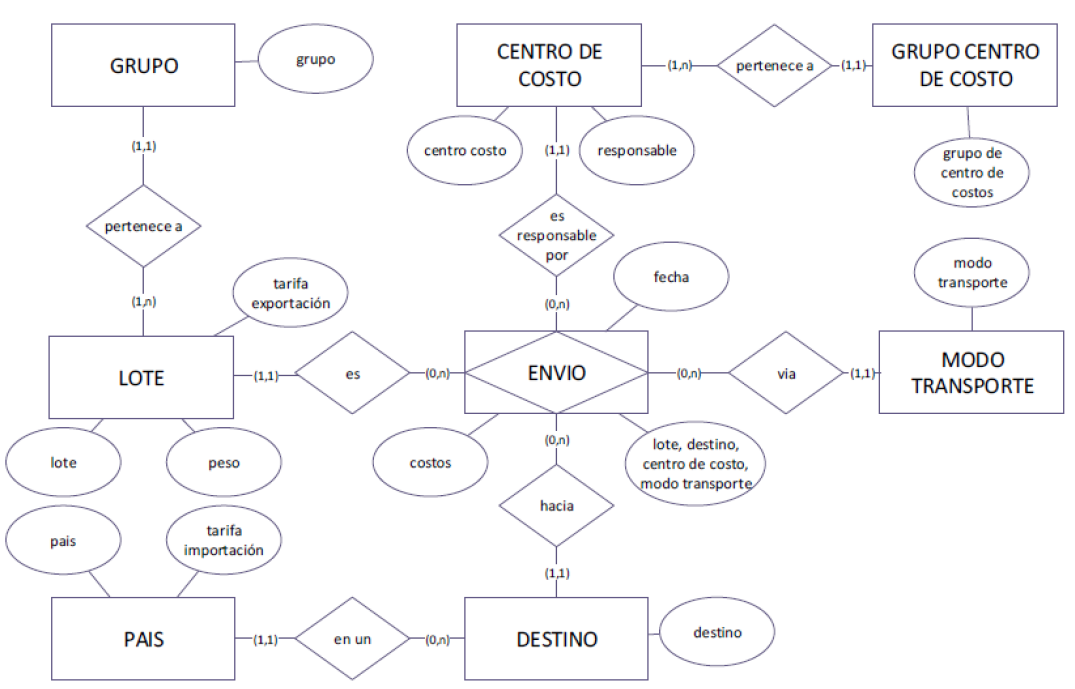
\includegraphics[width=11cm]{./images/Ejercicio_1}
			
		\end{center}
	\end{figure}

\subsubsection{\textbf{Diagrama E/R con Erwin }}

	\begin{figure}[htb]
		\begin{center}
			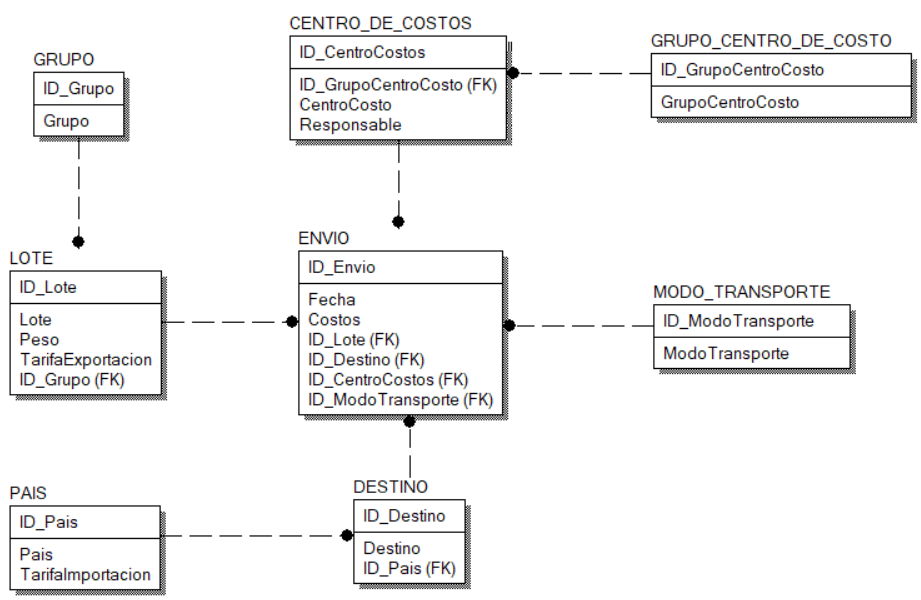
\includegraphics[width=12cm]{./images/erwin_1}
			
		\end{center}
	\end{figure}

%%\hfill \break
\newpage

\subsubsection{\textbf{Modelo Dimensional }}

	\begin{figure}[htb]
		\begin{center}
			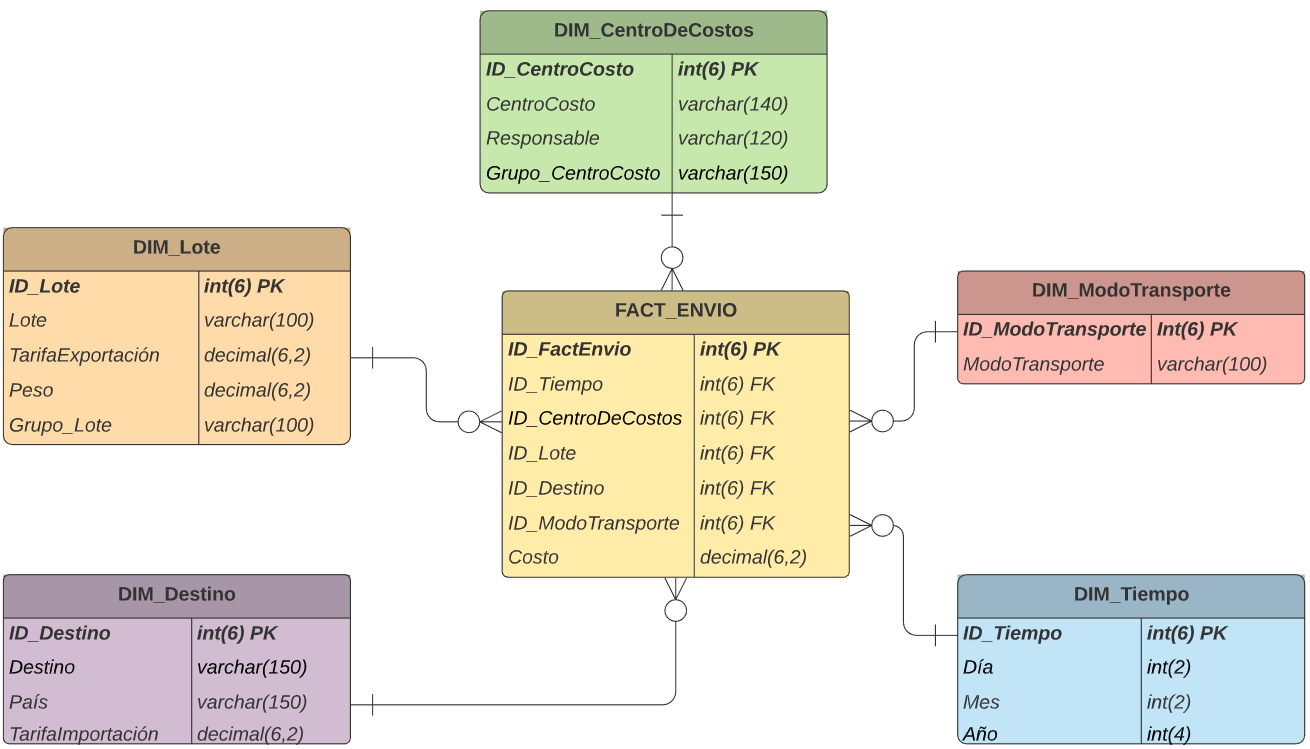
\includegraphics[width=12.5cm]{./images/mod_dimensional_1}
			
		\end{center}
	\end{figure}

\subsubsection{\textbf{Script SQL }}

	\begin{figure}[htb]
		\begin{center}
			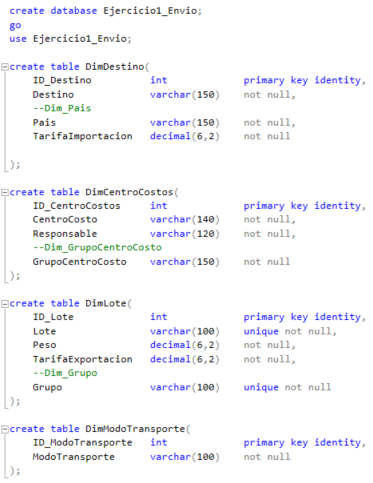
\includegraphics[width=6.5cm]{./images/Ejercicio1_script1}
			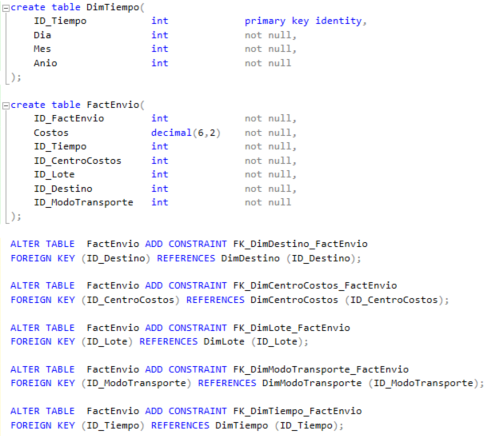
\includegraphics[width=8cm]{./images/Ejercicio1_script2}
		\end{center}
	\end{figure}
\newpage

\subsubsection{\textbf{Diagrama Físico }}

	\begin{figure}[htb]
		\begin{center}
			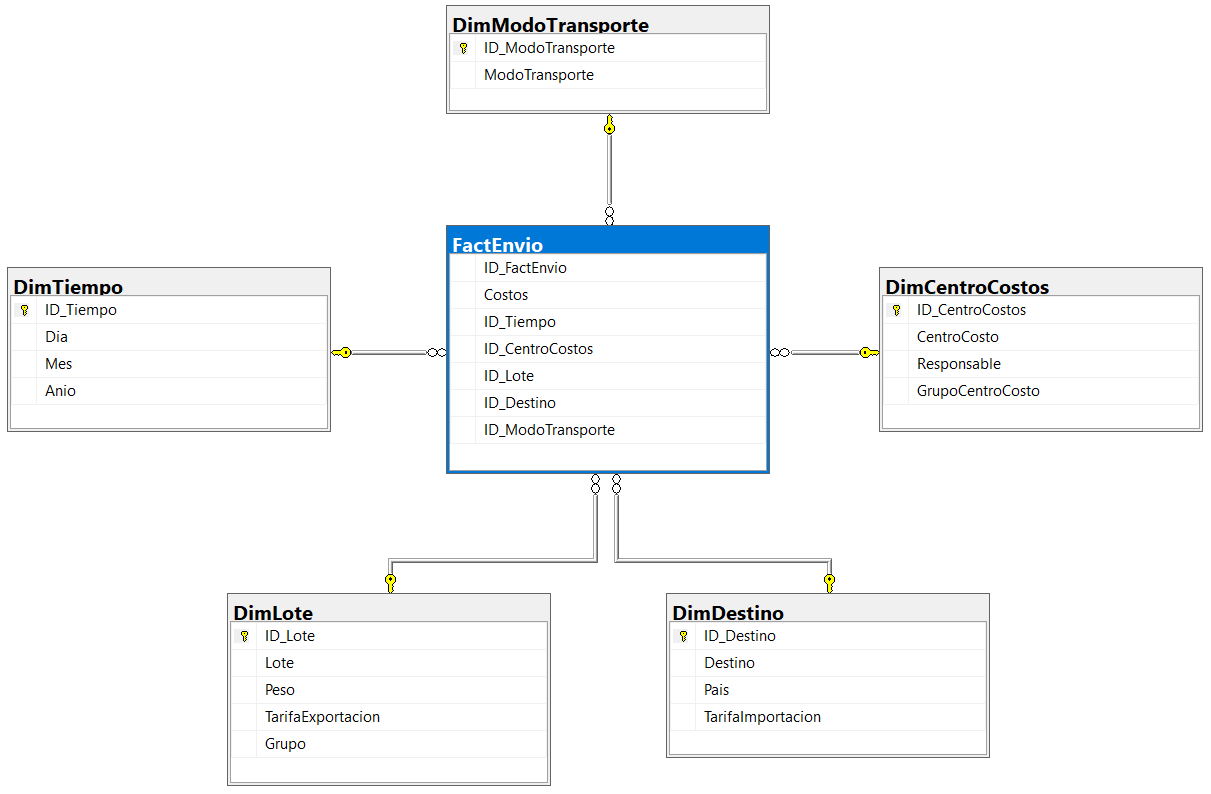
\includegraphics[width=15cm]{./images/Ejercicio1_DiagramaFisico}
			
		\end{center}
	\end{figure}

\newpage

%% EJERCICIO 2-------------------------------------------------------------------------------------------------------------------

\subsection{Ejercicio N° 02: Reservas de Viaje}

En este esquema de E / R, un cliente (que es de cierto tipo) reserva un viaje en una agencia de viajes. La agencia de viajes trabaja para un determinado operador turístico. El viaje va a un destino determinado que pertenece a un país determinado. La dimensión de tiempo consiste en mes, trimestre y año.



\subsubsection{\textbf{Diagrama E / R Simplificado}}

	\begin{figure}[htb]
		\begin{center}
			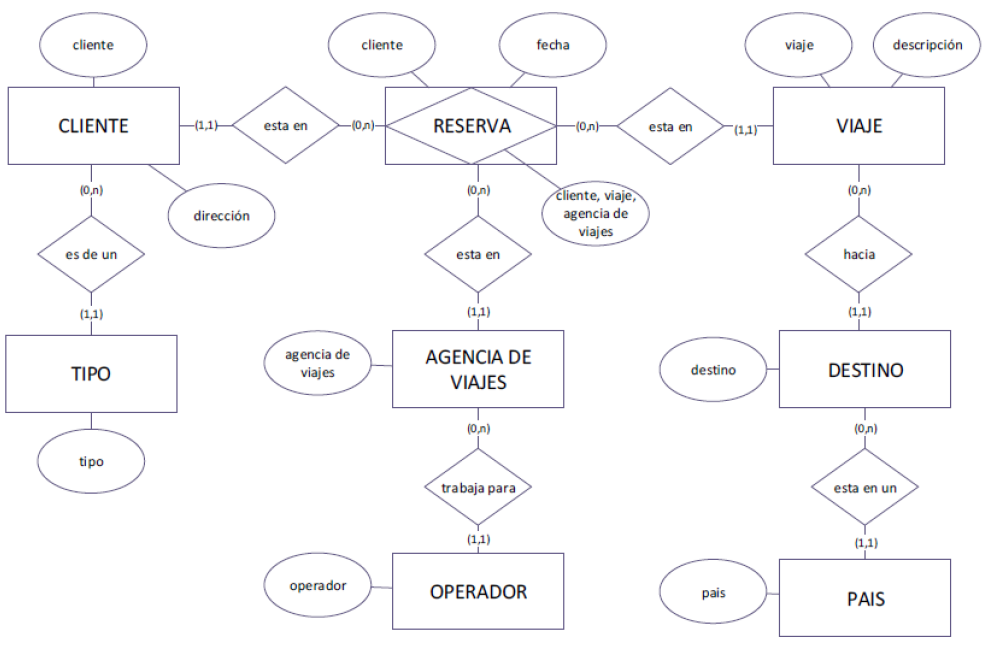
\includegraphics[width=11.5cm]{./images/Ejercicio_2}
			
		\end{center}
	\end{figure}

\subsubsection{\textbf{Diagrama E/R con Erwin}}

	\begin{figure}[htb]
		\begin{center}
			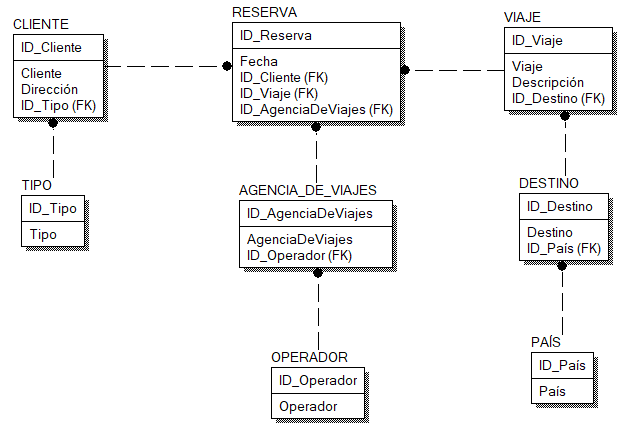
\includegraphics[width=12cm]{./images/erwin_2}
			
		\end{center}
	\end{figure}

%%\hfill \break
\newpage

\subsubsection{\textbf{Modelo Dimensional }}

	\begin{figure}[htb]
		\begin{center}
			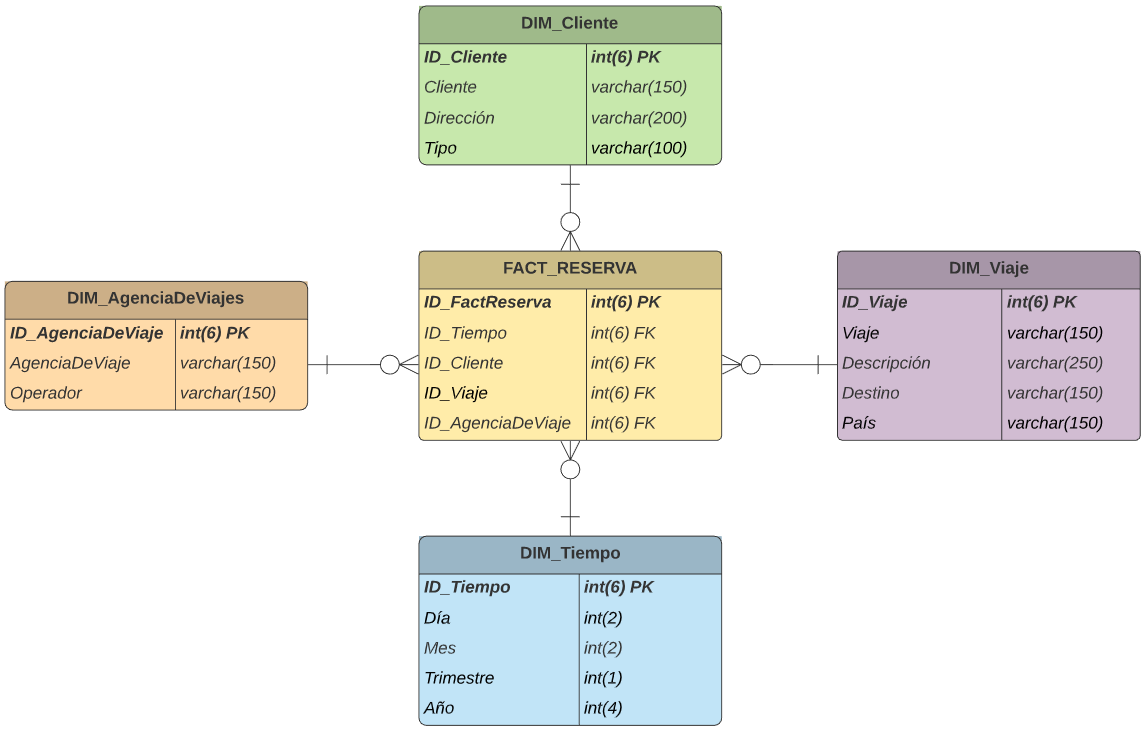
\includegraphics[width=14cm]{./images/mod_dimensional_2}
			
		\end{center}
	\end{figure}

\subsubsection{\textbf{Script SQL }}

	\begin{figure}[htb]
		\begin{center}
			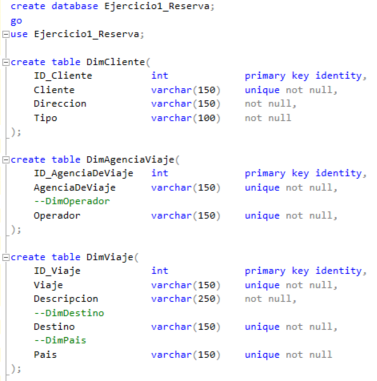
\includegraphics[width=6.5cm]{./images/Ejercicio2_script1}
			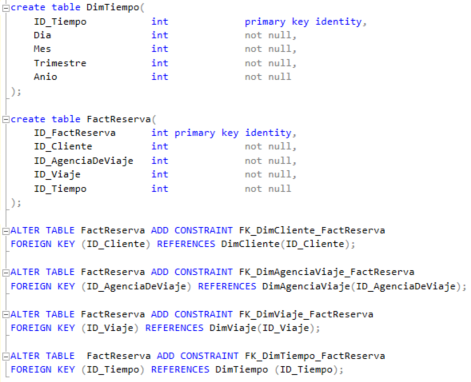
\includegraphics[width=8cm]{./images/Ejercicio2_script2}
		\end{center}
	\end{figure}

\newpage
\subsubsection{\textbf{Diagrama Físico }}

	\begin{figure}[htb]
		\begin{center}
			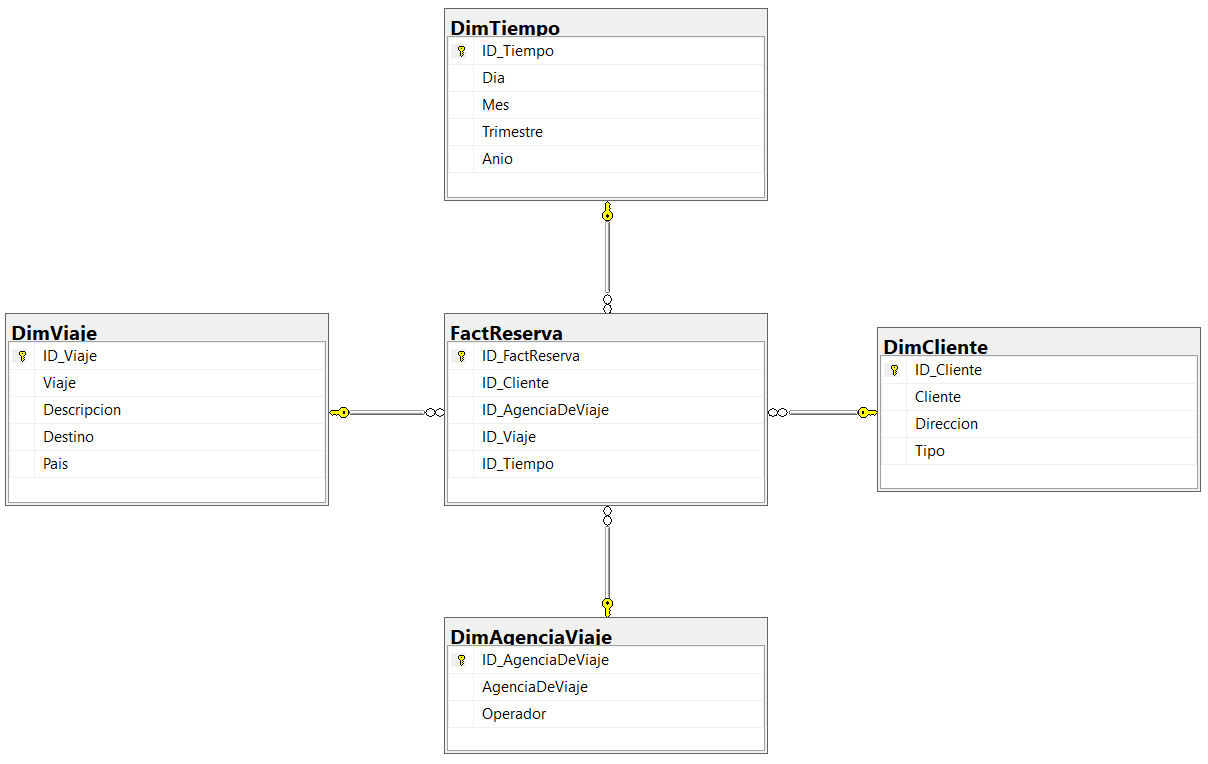
\includegraphics[width=15cm]{./images/Ejercicio2_DiagramaFisico}
			
		\end{center}
	\end{figure}

\newpage

%% EJERCICIO 3-------------------------------------------------------------------------------------------------------------------

\subsection{Ejercicio N° 03: Gestión de Proyectos}

Este esquema E / R simplificado muestra un caso gestión del proyecto. El proyecto para un cliente se divide en varios paquetes de trabajo y siempre una persona es responsable de completar la tarea. Se cuida en un lugar determinado. La dimensión de tiempo consiste de día, mes y año.

\subsubsection{\textbf{Diagrama E / R Simplificado}}

	\begin{figure}[htb]
		\begin{center}
			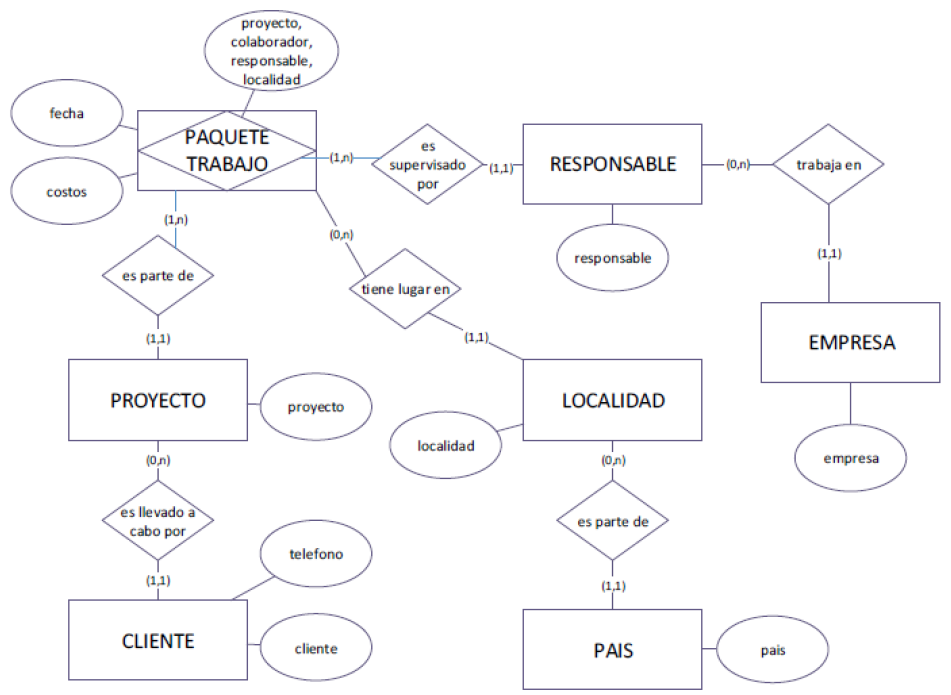
\includegraphics[width=11cm]{./images/Ejercicio_3}
			
		\end{center}
	\end{figure}

\subsubsection{\textbf{Diagrama E/R con Erwin }}

	\begin{figure}[htb]
		\begin{center}
			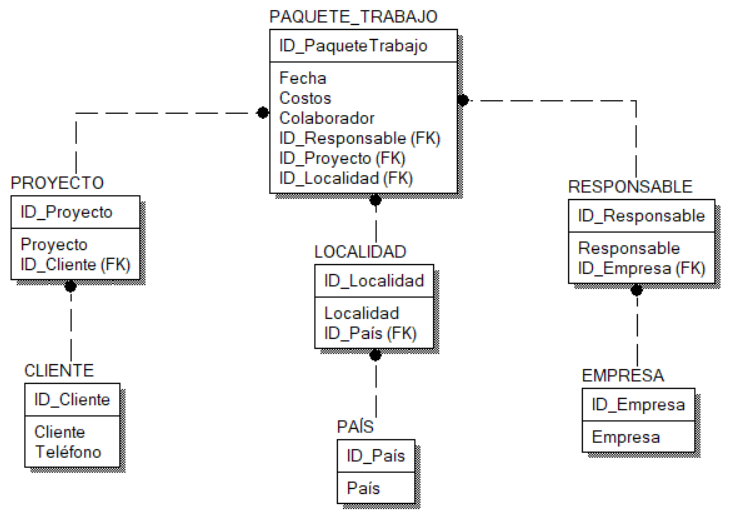
\includegraphics[width=12cm]{./images/erwin_3}
			
		\end{center}
	\end{figure}

%%\hfill \break
\newpage

\subsubsection{\textbf{Modelo Dimensional }}

	\begin{figure}[htb]
		\begin{center}
			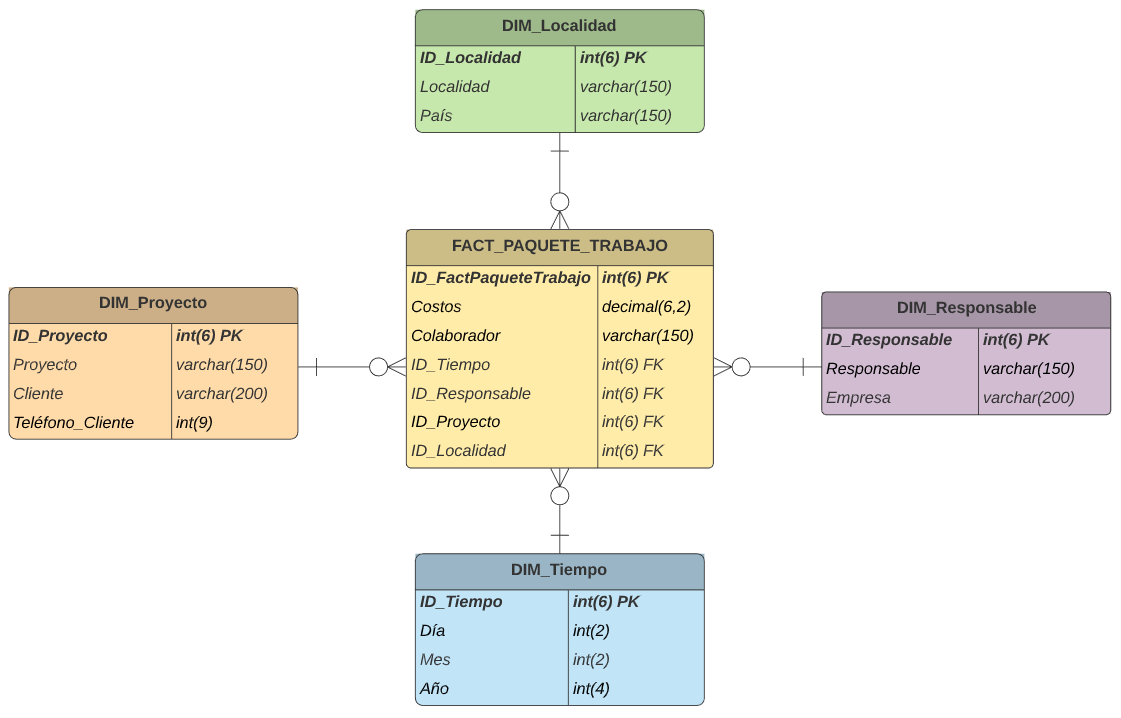
\includegraphics[width=14cm]{./images/mod_dimensional_3}
			
		\end{center}
	\end{figure}

\subsubsection{\textbf{Script SQL }}

	\begin{figure}[htb]
		\begin{center}
			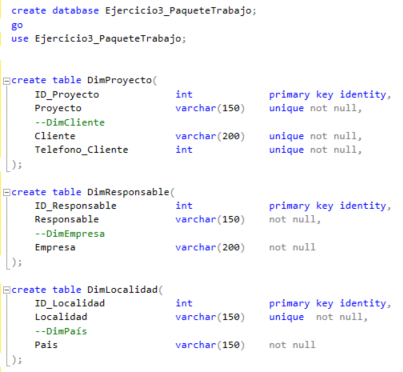
\includegraphics[width=6.5cm]{./images/Ejercicio3_script1}
			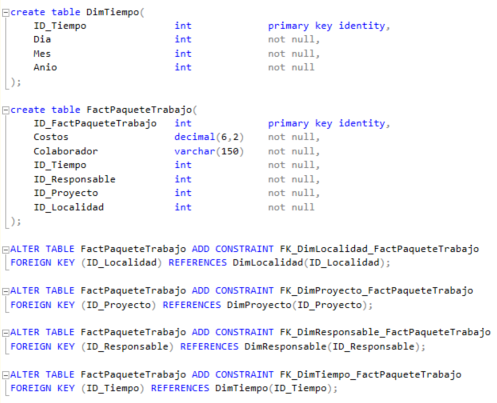
\includegraphics[width=8cm]{./images/Ejercicio3_script2}
		\end{center}
	\end{figure}
\newpage
\subsubsection{\textbf{Diagrama Físico }}

	\begin{figure}[htb]
		\begin{center}
			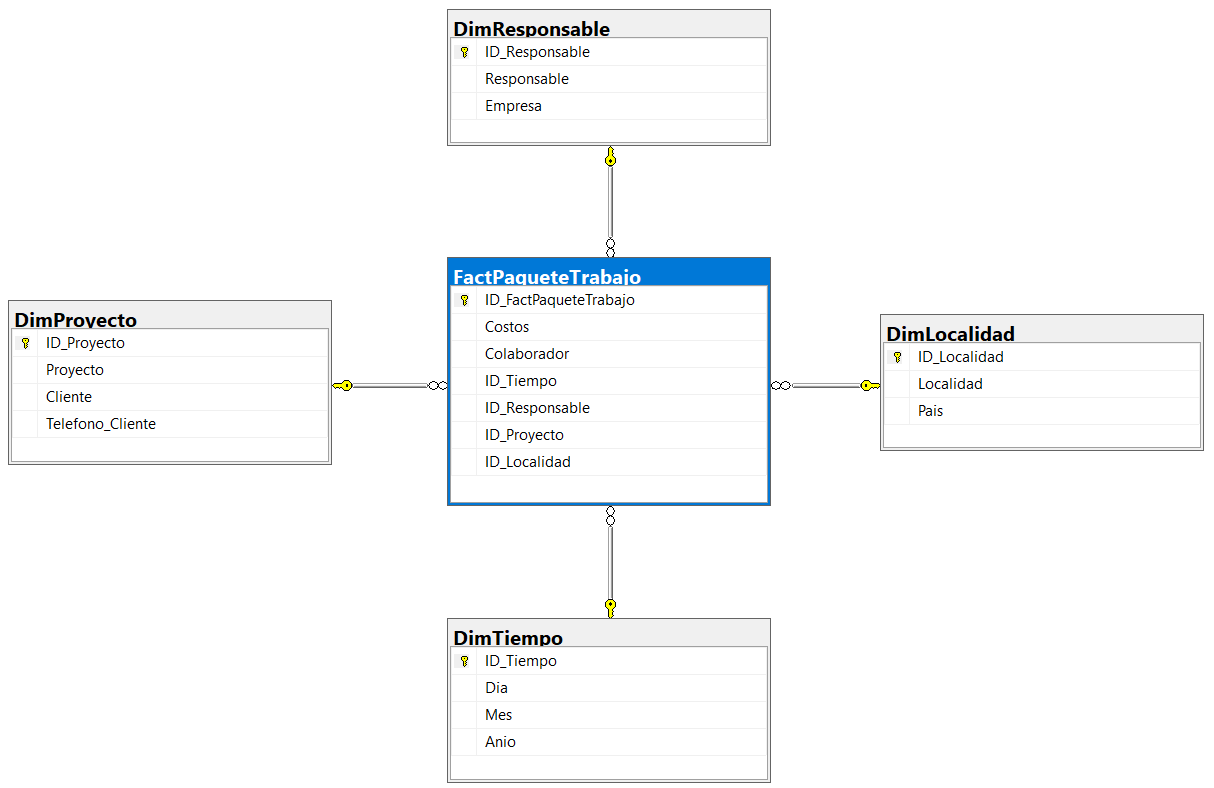
\includegraphics[width=12cm]{./images/Ejercicio3_DiagramaFisico}
			
		\end{center}
	\end{figure}

\newpage
\end{document}
